%% Retrieval Evaluation de Baeza
% - Introducción.
% - Retrieval performance.
% - Más...

Conociendo que ante la consulta de un usuario que presenta cierto grado de incertidumbre, la lista de documentos recuperados no será una respuesta exacta y determinística como ocurre en sistemas de bases de datos relacionales. Las medidas de evaluación propias de una sistema de recuperación de información nos permiten conocer la calidad de las respuestas del sistema ante determinadas consultas. Más allá de las medidas de rendimiento de cualquier sistema computacional, como el tiempo de respuesta o el espacio necesario para responder una consulta, que también se podrán tener en cuenta. \\

En este capítulo haremos foco sobre medidas específicas en la recuperación de información. Es importante mencionar que cuando se quiere medir la performance de un sistema hay que tener en claro la tarea de recuperación que realiza, la cual podrá consistir de consultas procesadas por lote (batch mode) o sino mediante una sesión interactiva donde el usuario irá especificando la información que necesita a través de una serie de pasos. Esta aclaración es para ilustrar que existen diferentes formas de procesamiento con lo cual la manera de evaluar su rendimiento también será diferente. \\

Muchas medidas de rendimiento y correctitud fueron propuesta, sólo veremos las tres que consideramos mas interesantes pero sepan que hay muchas más que se pueden aplicar quizás dependiendo el contexto en donde se utilice el sistema, para mas información puede consultar \cite{baeza2011} \\

Consideremos una consulta \textit{q} sobre una colección de documentos \textit{D} y una estrategia de recuperación \textit{S} a evaluar. Suponemos conocido el conjunto \textit{R} de documentos determinados como revelantes para el usuario ante la necesidad de información que representa la consulta \textit{q}, en este caso los documentos se clasifican como relevantes o no, en otro escenario es posible que la relevancia sea multivaluada. \\ \\ \\
Sea \textit{A} el conjunto ordenado de respuesta de un sistema aplicando la estrategia \textit{S} sobre la consulta \textit{q}, mientras que \textit{R} es el conjunto de todos los documentos de información revelantes para esa consulta.

	\begin{figure}[h]
		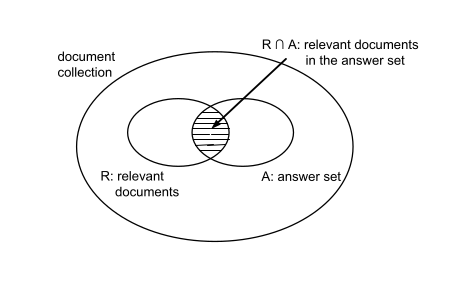
\includegraphics[width=8cm]{evaluation-retrieval}
		\centering
		\caption{Diagrama de conjuntos. (Figura extraída de \cite{baeza2011})}
	\end{figure}

\section{Precisión}
Esta medida define la fracción de los documentos recuperados que son relevantes para el usuario cuando realiza la consulta \textit{q}. Podemos considerar que cada documentos relevante recuperado es un acierto (hit) del sistema. \\

					\begin{equation}
						Precision = \cfrac{|R \cap A|}{|A|}
					\end{equation}
	
\section{Recall o Exhaustividad}
Esta medida define la proporción de los documentos relevantes que fueron recuperados para la consulta \textit{q}. Cada documento relevante no recuperado representa un desacierto (miss) del sistema. \\

					\begin{equation}
						Recall = \cfrac{|R \cap A|}{|R|}
					\end{equation}
					
Con esta dos medidas podemos definir una curva donde nos muestre el valor de precisión alcanzado por el sistema utilizando \textit{S} para ciertos valores de exhaustividad. \\
	
\section{Fall-out o Proporción de fallos}
La proporción de fallos define la fracción de los documentos no relevantes que fueron recuperados para una consulta. Representa la tasa de falsos positivos en el sistema.\\
Resulta deseable minimizar esta variable o maximizar la exhaustividad y al mismo tiempo lograr mayor precisión en las respuestas. \\
Siendo \textit{N} el tamaño de la colección de los documentos, podemos definir el índice de fallos como sigue:

					\begin{equation}
						Fall-out = \cfrac{|A - (R \cup A)|}{N - |R|}
					\end{equation}

%---Hablar sobre las medidas online y la diferencia con las medidas offline